\documentclass[11pt]{article}
\usepackage{tikz}
\usepackage{tikz-qtree}
%\usepackage{amsfonts}
\usetikzlibrary{automata, arrows, positioning}

\title{Homework \#3}
\author{Kyle White}
\date{March 11, 2017}

\begin{document}
\maketitle

\noindent2.1a) \\

\begin{tikzpicture}[level/.style={sibling distance=60mm/#1}]
%\node (0){$n$}
  %child {node (1) {$\frac{n}{2}$}
    %child {node (2) {$\frac{n}{2^2}$}
      %child {node (3) {baller}
        %child {node (4) {$\frac{n}{2^k}$}}
        %child {node (5) {$\frac{n}{2^k}$}}
      %} 
      %child {node (6) {hi}
				%child {node (7) {child}}
			%}
    %}
    %child {node [circle,draw] (8) {$\frac{n}{2^2}$}
      %child {node (9) {$\vdots$}}
      %child {node (10) {$\vdots$}}
    %}
  %};
%%\path (b) -- (g) node [midway] {+};
%%\path (d) -- (e) node [midway] {+};

\node (0) {E}
	child {node (1) {T}
		child {node (2) {F}
			child {node (3) {a}
			}
		}
	};

\end{tikzpicture}

\noindent2.1b) \\
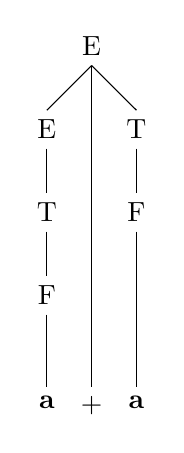
\begin{tikzpicture}
  [
    every tree node/.style={align=center,anchor=north},
    frontier/.style={distance from root=130pt}
  ]
  \Tree
  [.{E}
    [.{E}
      [.{T}
        [.{F} \textbf{a} ]
      ]
		]
    [ + ]
    [.{T}
      [.{F} \textbf{a} ]
    ]
  ]
\end{tikzpicture}

\noindent 2.1c) \\
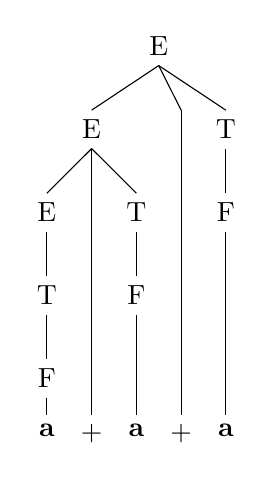
\begin{tikzpicture}
  [
    every tree node/.style={align=center,anchor=north},
    frontier/.style={distance from root=140pt}
  ]
  \Tree
  [.{E}
    [.{E}
			[.{E}
				[.{T}
					[.{F} \textbf{a} ]
				]
			]
			[ + ]
			[.{T}
				[.{F} \textbf{a} ]
			]
		]
		[ + ]
		[.{T}
			[.{F} \textbf{a} ]
		]
	]
\end{tikzpicture}

\noindent 2.1d) \\
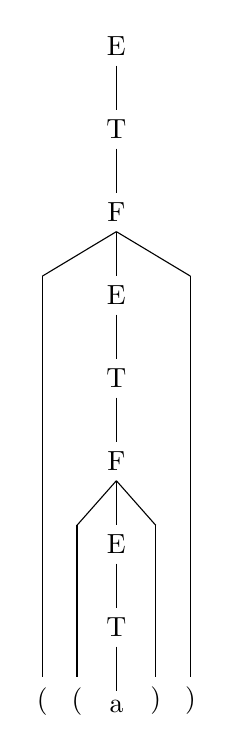
\begin{tikzpicture}
  [
    every tree node/.style={align=center,anchor=north},
    frontier/.style={distance from root=235pt}
  ]
  \Tree
  [.{E}
    [.{T}
			[.{F}
				[{(} ]
				[.{E}
					[.{T}
						[.{F}
						[{(} ]
							[.{E}
								[.{T}
									[.{a} ]
								]
							]
							[{)} ]
						]
					]
				]
				[{)} ]
			]
		]
	]
\end{tikzpicture}

\noindent2.4b) \\
$S \to 0P0 \vert 1P1 \vert$ \\
$P \to 0P \vert 1P \vert \epsilon$ \\

\noindent2.4c) \\
$S \to 0 \vert 1 \vert 0S0 \vert 0S1 \vert 1S0 \vert 1S1$ \\

\noindent2.4e) \\
$S \to 0 \vert 1 \vert 0S0 \vert 1S1 \vert \epsilon$ \\

\noindent2.4f) \\
$S \to S$ \\

\noindent2.5a) \\
Informal Description: This grammar is simple in the sense that it does not require a stack.  As long as a string has at least three 1s, the push down automata will accept. \\
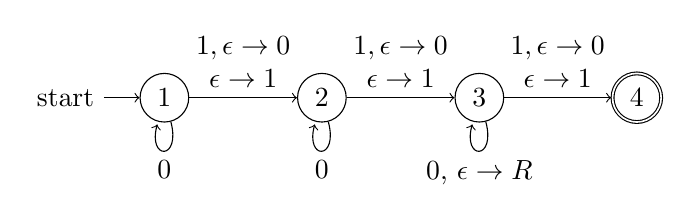
\begin{tikzpicture}

\tikzset{vertex/.style = {shape=circle,draw,minimum size=1em}}
\tikzset{edge/.style = {->,> = latex'}}
% vertices
\node[vertex, initial] (1) at  (0,0) {1};
\node[vertex] (2) at  (2,0) {2};
\node[vertex] (3) at  (4,0) {3};
\node[vertex, accepting] (4) at (6,0) {4};
%edges

\draw [->] (1) -- (2) node [align=center, midway, above] {$1, \epsilon \to 0$\\$\epsilon \to 1$};
\draw [->] (2) -- (3) node [align=center, midway, above] {$1, \epsilon \to 0$\\$\epsilon \to 1$};
\draw [->] (3) -- (4) node [align=center, midway, above] {$1, \epsilon \to 0$\\$\epsilon \to 1$};
%\draw [->] (2) edge[bend left] node [label=below: {u}] {} (1);
\path (1) edge[loop below] node {0} (1);
\path (2) edge[loop below] node {0} (2);
\path (3) edge[loop below] node {0, $\epsilon \to R$} (3);

\end{tikzpicture}

\noindent2.5b) \\
\textbf{Informal Description: }This grammar recognizes any language that starts and ends with the same symbol.  The start symbol is pushed on to the stack and nothing is popped until the same symbol has been seen again.
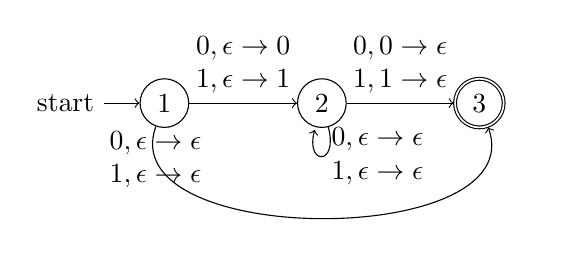
\begin{tikzpicture}

\tikzset{vertex/.style = {shape=circle,draw,minimum size=1em}}
\tikzset{edge/.style = {->,> = latex'}}
% vertices
\node[vertex, initial] (1) at  (0,0) {1};
\node[vertex] (2) at  (2,0) {2};
\node[vertex, accepting] (3) at  (4,0) {3};
%edges
\draw [->] (1) -- (2) node [align=center, midway, above] {$0, \epsilon \to 0$\\$1, \epsilon \to 1$};
\draw [->] (2) -- (3) node [align=center, midway, above] {$0, 0 \to \epsilon$\\$1, 1 \to \epsilon$};
\draw [->] (1) edge[bend right=110] node [align=center, midway, pos=0.1] {$0, \epsilon \to \epsilon$\\$1, \epsilon \to \epsilon$} (3);
\path (2) edge[loop below] node [align=center, right] {$0, \epsilon \to \epsilon$\\$1, \epsilon \to \epsilon$} (2);
%\path (3) edge[loop below] node {0, $\epsilon \to R$} (3);
\end{tikzpicture}

\noindent2.5c) \\
\textbf{Informal Description: }This grammar does not require a stack because odd length inputs do not require memory. In other words, it is not necessary to remember what input has already been read because as long as the length of the input is odd, it does not matter what has been read before. \\
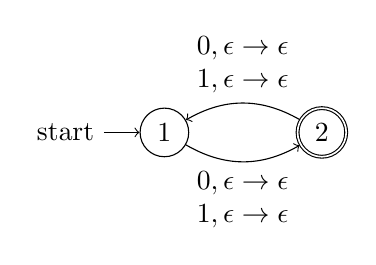
\begin{tikzpicture}

\tikzset{vertex/.style = {shape=circle,draw,minimum size=1em}}
\tikzset{edge/.style = {->,> = latex'}}
% vertices
\node[vertex, initial] (1) at  (0,0) {1};
\node[vertex, accepting] (2) at  (2,0) {2};
%edges
%\draw [->] (1) -- (2) node [align=center, midway, above] {$0, \epsilon \to \epsilon$\\$1, \epsilon \to \epsilon$};
%\draw [->] (2) -- (1) node [align=center, midway, below] {$0, \epsilon \to \epsilon$\\$1, \epsilon \to \epsilon$};
\draw [->] (2) edge[bend right] node [align=center, midway, above] {$0, \epsilon \to \epsilon$\\$1, \epsilon \to \epsilon$} (1);
\draw [->] (1) edge[bend right] node [align=center, midway, below] {$0, \epsilon \to \epsilon$\\$1, \epsilon \to \epsilon$} (2);
%\path (2) edge[loop below] node [align=center, right] {$0, \epsilon \to \epsilon$\\$1, \epsilon \to \epsilon$} (2);
%\path (3) edge[loop below] node {0, $\epsilon \to R$} (3);
\end{tikzpicture}

\noindent2.5d) \\
\textbf{Informal Description: }For this grammar, a symbol is pushed on at the beginning of the input.  When the middle of the input is hit, a 0 will be pushed on to the stack.  The stack is then popped for the same amount of pushes on the stack before the 0.  If there is no input left and 0 is the middle of the input, the symbol pushed at the start of the input is now popped and the PDA accepts. Otherwise, the PDA rejects. \\
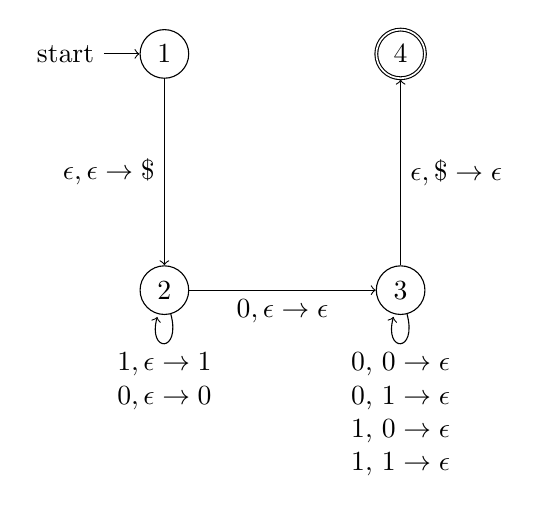
\begin{tikzpicture}

\tikzset{vertex/.style = {shape=circle,draw,minimum size=1em}}
\tikzset{edge/.style = {->,> = latex'}}
% vertices
\node[vertex, initial] (1) at  (0,0) {1};
\node[vertex] (2) at  (0,-3) {2};
\node[vertex] (3) at  (3,-3) {3};
\node[vertex, accepting] (4) at  (3,0) {4};
%edges
\draw [->] (1) -- (2) node [align=center, midway, left] {$\epsilon, \epsilon \to \$$};
\draw [->] (2) -- (3) node [align=center, midway, below] {$0, \epsilon \to \epsilon$};
\draw [->] (3) -- (4) node [align=center, midway, right] {$\epsilon, \$ \to \epsilon$};
%\draw [->] (2) -- (1) node [align=center, midway, below] {$0, \epsilon \to \epsilon$\\$1, \epsilon \to \epsilon$};
%\draw [->] (2) edge[bend right] node [align=center, midway, above] {$0, \epsilon \to \epsilon$\\$1, \epsilon \to \epsilon$} (1);
%\draw [->] (1) edge[bend right] node [align=center, midway, below] {$0, \epsilon \to \epsilon$\\$1, \epsilon \to \epsilon$} (2);
\path (2) edge[loop below] node [align=center, below] {$1, \epsilon \to 1$\\$0, \epsilon \to 0$} (2);
\path (3) edge[loop below] node [align=center, below] {0, $0 \to \epsilon$\\0, $1 \to \epsilon$\\1, $0 \to \epsilon$\\1, $1 \to \epsilon$} (3);
\end{tikzpicture}

\noindent2.5e) \\
\textbf{Informal Description: }For this grammar, the input represented is a palindrome.  The beginning of the palindrome is pushed on to the stack.  Once the middle is reached, the remaining input must mirror the exact first half of the palindrome and pop off the stack in that order.  If the stack is empty at the end of the input, the PDA accepts.  Otherwise, it rejects. \\
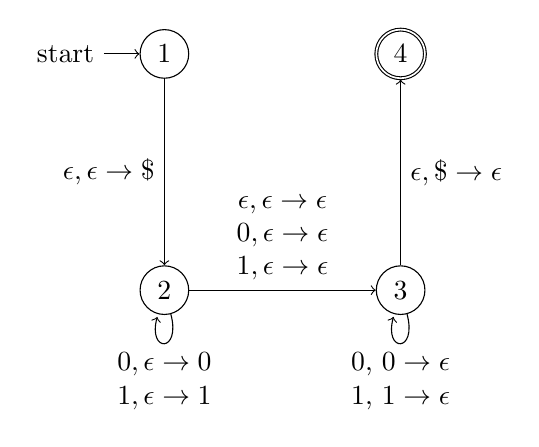
\begin{tikzpicture}

\tikzset{vertex/.style = {shape=circle,draw,minimum size=1em}}
\tikzset{edge/.style = {->,> = latex'}}
% vertices
\node[vertex, initial] (1) at  (0,0) {1};
\node[vertex] (2) at  (0,-3) {2};
\node[vertex] (3) at  (3,-3) {3};
\node[vertex, accepting] (4) at  (3,0) {4};
%edges
\draw [->] (1) -- (2) node [align=center, midway, left] {$\epsilon, \epsilon \to \$$};
\draw [->] (2) -- (3) node [align=center, midway, above] {$\epsilon, \epsilon \to \epsilon$\\$0, \epsilon \to \epsilon$\\$1, \epsilon \to \epsilon$};
\draw [->] (3) -- (4) node [align=center, midway, right] {$\epsilon, \$ \to \epsilon$};
%\draw [->] (2) -- (1) node [align=center, midway, below] {$0, \epsilon \to \epsilon$\\$1, \epsilon \to \epsilon$};
%\draw [->] (2) edge[bend right] node [align=center, midway, above] {$0, \epsilon \to \epsilon$\\$1, \epsilon \to \epsilon$} (1);
%\draw [->] (1) edge[bend right] node [align=center, midway, below] {$0, \epsilon \to \epsilon$\\$1, \epsilon \to \epsilon$} (2);
\path (2) edge[loop below] node [align=center, below] {$0, \epsilon \to 0$\\$1, \epsilon \to 1$} (2);
\path (3) edge[loop below] node [align=center, below] {0, $0 \to \epsilon$\\1, $1 \to \epsilon$} (3);
\end{tikzpicture}

\noindent2.5f) \\
\textbf{Informal Description: }This grammar recognizes the empty set so it does not accept any strings. \\
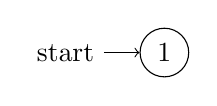
\begin{tikzpicture}

\tikzset{vertex/.style = {shape=circle,draw,minimum size=1em}}
\tikzset{edge/.style = {->,> = latex'}}
% vertices
\node[vertex, initial] (1) at  (0,0) {1};

\end{tikzpicture}

\noindent2.6b)\\
$S \to S_1 | S_2$ \\
$S_1 \to aS_1b | A | B$ \\
$S_2 \to CbaC$ \\
$A \to aA | a$ \\
$B \to Bb | b$ \\
$C \to CC | a | b | \epsilon$ \\

\noindent2.6d)\\
$S \to aSa | bSb | \# | \#A\#$\\
$A \to aA|bA|\#A|\epsilon$\\
$B \to S|A\#S\#A|A\#S|S\#A$\\

\noindent2.9)\\
$S \to S_1|S_2$\\
$S_1 \to S_1c|A|\epsilon$\\
$S_2 \to aS_2|B|\epsilon$\\
$A \to aAb|\epsilon$\\
$B \to bBc|\epsilon$\\ \\
The CFG is ambiguous because it can be derived using $S_1$ or $S_2$.

\noindent2.10)\\
To design this PDA, you can split the language into two individual languages and combine them at the end.  The final PDA will be described as follows: Start by either reading in a's and pushing them on the stack or by skipping them all together.  If you read in a's, then read in b's and for each b, pop an a off of the stack.  If the stack is empty when the the b's have all been processed, skip the remaining c's and accept the language.  If you skipped reading in a's, read in b's and push them on to the stack.  Then, read in c's and for each c read, pop a b off of the stack.  If there are no more b's on the stack when the c's have finished being read, the language will be accepted.\\

\noindent2.11)\\
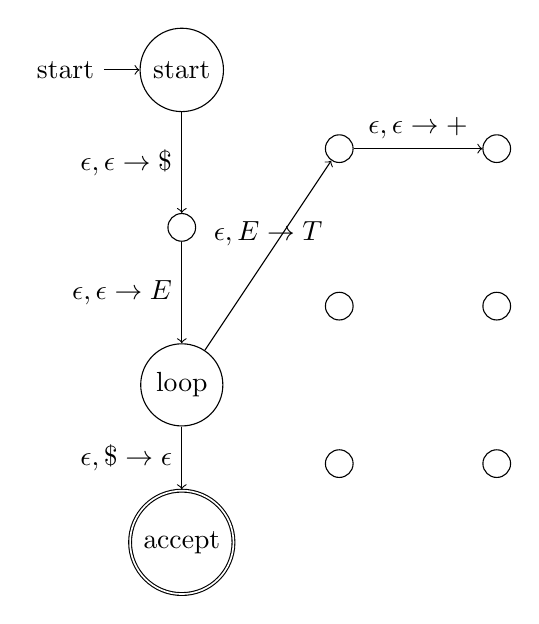
\begin{tikzpicture}

\tikzset{vertex/.style = {shape=circle,draw,minimum size=1em}}
\tikzset{edge/.style = {->,> = latex'}}
% vertices
\node[vertex, initial] (1) at  (0,4) {start};
\node[vertex] (2) at  (0,2) {};
\node[vertex] (3) at  (0,0) {loop};
\node[vertex, accepting] (4) at  (0,-2) {accept};
\node[vertex] (5) at  (2,3) {};
\node[vertex] (6) at  (4,3) {};
\node[vertex] (7) at  (2,1) {};
\node[vertex] (8) at  (4,1) {};
\node[vertex] (9) at  (2,-1) {};
\node[vertex] (10) at  (4,-1) {};
%edges
\draw [->] (1) -- (2) node [align=center, midway, left] {$\epsilon, \epsilon \to \$$};
\draw [->] (2) -- (3) node [align=center, midway, left] {$\epsilon, \epsilon \to E$};
\draw [->] (3) -- (4) node [align=center, midway, left] {$\epsilon, \$ \to \epsilon$};
\draw [->] (3) -- (5) node [align=center, midway, above] {$\epsilon, E \to T$};
\draw [->] (5) -- (6) node [align=center, midway, above] {$\epsilon, \epsilon \to +$};
%\draw [->] (2) -- (3) node [align=center, midway, above] {$\epsilon, \epsilon \to \epsilon$\\$0, \epsilon \to \epsilon$\\$1, \epsilon \to \epsilon$};
%\draw [->] (3) -- (4) node [align=center, midway, right] {$\epsilon, \$ \to \epsilon$};
%%\draw [->] (2) -- (1) node [align=center, midway, below] {$0, \epsilon \to \epsilon$\\$1, \epsilon \to \epsilon$};
%%\draw [->] (2) edge[bend right] node [align=center, midway, above] {$0, \epsilon \to \epsilon$\\$1, \epsilon \to \epsilon$} (1);
%%\draw [->] (1) edge[bend right] node [align=center, midway, below] {$0, \epsilon \to \epsilon$\\$1, \epsilon \to \epsilon$} (2);
%\path (2) edge[loop below] node [align=center, below] {$0, \epsilon \to 0$\\$1, \epsilon \to 1$} (2);
%\path (3) edge[loop below] node [align=center, below] {0, $0 \to \epsilon$\\1, $1 \to \epsilon$} (3);
%TODO: Finish 2.11
\end{tikzpicture}

\noindent2.12)\\
%TODO: Finish this problem

\noindent2.13)\\
L(G) has a couple of different rules for languages that are recognized.  The first is that you can have two $\#$s in the middle of an infinite amount of 0s on either side of them.  The other is that you can have 1 $\#$ and the number of 0s on the left of the $\#$ must be 1/2 the number of 0s on the right side of the $\#$. \\
%TODO: Finish part b of this problem

\noindent2.14)\\
Add Start Variable \\
$S_0 \to A$\\
$A \to BAB | B | \epsilon$\\
$B \to 00 | \epsilon$\\ \\

Remove all $\epsilon$\\
$S_0 \to A|\epsilon$\\
$A\to BAB|BA|AB|A|B|BB$\\
$B \to 00$\\

Remove unit rules\\
$S_0 \to BAB|BA|AB|00|BB|\epsilon$\\
$A \to BAB|BA|AB|00|BB$\\
$B \to 00$\\

Replace terminals with new variables\\
$S_0 \to BAB|BA|AB|UU|BB|\epsilon$\\
$A \to BAB|BA|AB|UU|BB$\\
$B \to UU$\\
$U \to 0$\\

Shorten RHS\\
$S_0 \to BA_1|BA|AB|UU|BB|\epsilon$\\
$A \to BA_2|BA|AB|UU|BB$\\
$B \to UU$\\
$U \to 0$\\
$A_1 \to AB$\\
$A_2 \to AB$\\

\noindent2.26)\\
%TODO: Finish this

\noindent2.30)\\


\end{document}